\documentclass[12pt,twocolumn]{article}
\usepackage[T1]{fontenc}
\usepackage{graphicx}
\usepackage{tabularx}
\usepackage{amsmath,amsthm,amssymb}
%\usepackage{esvect}
\usepackage[left=2cm,right=2cm,top=2.5cm,bottom=2.5cm]{geometry}
%\renewcommand*{\familydefault}{\sfdefault}
\newcommand{\st}[0]{\text{*}}
\title{\textbf{Driven Cavity with SIMPLE}}
\author{Christopher Pattison}
\date{}
\begin{document}

\twocolumn[
\begin{@twocolumnfalse}
\maketitle
\begin{abstract}
The finite volume method is applied to the incompressible, steady Navier-Stokes equations with
SIMPLE used to solve the resulting nonlinear system of equations for a driven cavity.
A term proposed by Rhie and Chow is added to the pressure correction to allow a collocated grid discretization.
Reynolds numbers from 10 to 400 were tested with changes in the solution due to viscosity observed.
\vspace{.5em}
\end{abstract}
\end{@twocolumnfalse}]

\section*{Introduction}
The driven cavity is a two-dimensional, incompressible fluid problem.
Solutions must satisfy the conservation of momentum \eqref{eq:navierstokes} and mass \eqref{eq:massconservation} as well as the boundary conditions \eqref{eq:boundarycondition}.
\begin{equation}\label{eq:navierstokes}\nabla\cdot\rho\vec u\vec u - \mu\nabla^2\vec u = -\nabla P\end{equation}
\begin{equation}\label{eq:massconservation}\nabla\cdot\vec u = 0\end{equation}
\begin{equation}\label{eq:boundarycondition}u|_e = u|_w = u|_s = 0\end{equation}
\[u|_n = 1\]
\[v|_e=v|_w=v|_n=v|_s=0\]
\[\left.\frac{\partial P}{\partial x}\right|_e=\left.\frac{\partial P}{\partial x}\right|_w=\left.\frac{\partial P}{\partial y}\right|_n=\left.\frac{\partial P}{\partial y}\right|_s=0\]
A finite volume method discretization is used with a nonlinear equation solver.

\subsubsection*{SIMPLE}
The SIMPLE algorithm solves the equations by perturbing a mass conserving solution towards momentum conservation and correcting the pressure field such that the momentum conserving solution also conserves mass. The steps are detailed as follows.

\begin{enumerate}
\item Initialize conservative guess for $u$ and $P$
\item Solve momentum conservation for $u\st$, the momentum conserving solution
\item Solve the pressure correction equation for $P'$, the pressure correction
\item Under-relax $P'$
\item Solve correction equation for $u'$, the velocity correction
\item Correct $u$ and $P$
\begin{itemize}
	\item $u$ = $u\st$ + $u'$
	\item $P$ = $P\st$ + $P'$
\end{itemize}
\item Go to 2 if not converged
\end{enumerate}
%TODO: Add boundary conditions and nice figure
%TODO: 2D structured grid is never stated

\section*{Methods}
The equations are discretized with the application of the finite volume method on a 2-dimensional, structured grid then manipulated to obtain the equations solved in SIMPLE.
\subsection*{Momentum}
The momentum equation is a convection-diffusion equation for the transport of a vector quantity.
Because of this, the discretization of the momentum equation is identical to that of a convection-diffusion equation with source term.
Application of the finite volume method results in equation \eqref{eq:nsfvm}.
\begin{equation}\label{eq:nsfvm}\sum\limits_n \vec S_n\cdot(\rho\vec u\vec u-\mu\nabla\vec u)_n= -\int_V\nabla p \hspace{.5ex}dV\end{equation} %Expand equation and add approximations?
\subsubsection*{Diffusion}
An approximation for the cell face gradient must be selected.
A finite differences approximation \eqref{eq:difference} of the gradient is easy and will provide sufficient accuracy.
\begin{equation}\label{eq:difference}\nabla\phi_e = \frac{\phi_E - \phi_P}{\vec x_E - \vec x_P}\end{equation}
%This results in equation \eqref{eq:diffusion} on a uniform structured grid.
%\begin{equation}\label{eq:diffusion}-\mu\left(\frac{u_E-2u_P+u_W}{\delta x} + \frac{u_N-2u_P+u_S}{\delta y}\right)\end{equation}

\subsubsection*{Convection}
The Peclet number can be defined as the ratio \eqref{eq:peclet} of convective and diffusive fluxes \eqref{eq:FD}.
\begin{equation}\label{eq:FD}F=\vec n\cdot\rho\vec u;\hspace{.5ex}D=\frac{\mu}{\delta x}\end{equation} %TODO: verify
\begin{equation}\label{eq:peclet}P = \frac{F}{D} = \frac{\rho u \delta x}{\mu}\end{equation}
This is useful to characterize how convective a problem is and will be used in the selection of interpolation functions for convective terms.

A linear interpolation \eqref{eq:linear} can result in negative coefficients and oscillations in the solution. Consequently, it cannot be used for convection dominated problems ($|P|>2$).
\begin{equation}\label{eq:linear}\phi_e = \frac{\phi_E + \phi_P}{2}\end{equation}
Simply taking the value of the field at the upwind node \eqref{eq:upwind} will unconditionally result in positive coefficients.
\begin{equation}\label{eq:upwind}\phi_e = \begin{cases}\phi_P & \vec u_e \cdot \vec n_e > 0\\\phi_E &\vec u_e \cdot \vec n_e \leq 0\end{cases}\end{equation}
Upwind interpolations work well for extremely convective flows but result an overly diffusive solution due to their low order of accuracy $O(h)$.
%TODO: add convection discretization

The coefficients resulting from an upwind discretization \eqref{eq:diffconvcoeff} can be weighted to allow different interpolation functions to be selected.
Usage of functions \eqref{eq:Alin} and \eqref{eq:Aupw} will result in a linear and upwind interpolation, respectively.
Function \eqref{eq:Apwr}, the so-called Power-law, will result in a smooth transition from a linear to an upwind interpolation scheme.
\begin{equation}\label{eq:Alin}A(P) = 1 - \frac 1 2 |P|\end{equation}
\begin{equation}\label{eq:Aupw}A(P) = 1\end{equation}
\begin{equation}\label{eq:Apwr}A(P) = \left\lceil 0, \left(1-\frac{|P|}{10}\right)^5 \hspace{.3ex}\right\rceil\end{equation}
\subsubsection*{Coefficients}

The coefficients resulting from discretizing the convection and diffusion terms are detailed below.
\begin{equation}\label{eq:diffconvcoeff}a_P^u u_P - \sum\limits_na_n^u u_n= b^u \end{equation}
\[a_E^u = D_eA(P_e) + \lceil -F_e, 0 \rceil\]
\[a_W^u = D_wA(P_w) + \lceil F_w, 0 \rceil\]
\[a_N^u = D_nA(P_n) + \lceil -F_n, 0 \rceil\]
\[a_S^u = D_sA(P_s) + \lceil F_s, 0 \rceil\]
\[a_P^u = \sum\limits_n a_n^u + F_e - F_w + F_n - F_s\]
Conveniently, the left hand sight of the momentum equation results in the same coefficients for each of the components of $\vec u$.
\[a^u = a^v\]

\subsubsection*{Source Term}
The source term is simply integrated over the control volume using equation \eqref{eq:difference} for the gradient reconstruction resulting in equations \eqref{eq:umomentsource} and \eqref{eq:vmomentsource}.
\begin{equation}\label{eq:umomentsource}b^u = -V \frac{P_E-P_W}{\delta x}\end{equation}
\begin{equation}\label{eq:vmomentsource}b^v = -V \frac{P_N-P_S}{\delta y}\end{equation}

\begin{figure*}
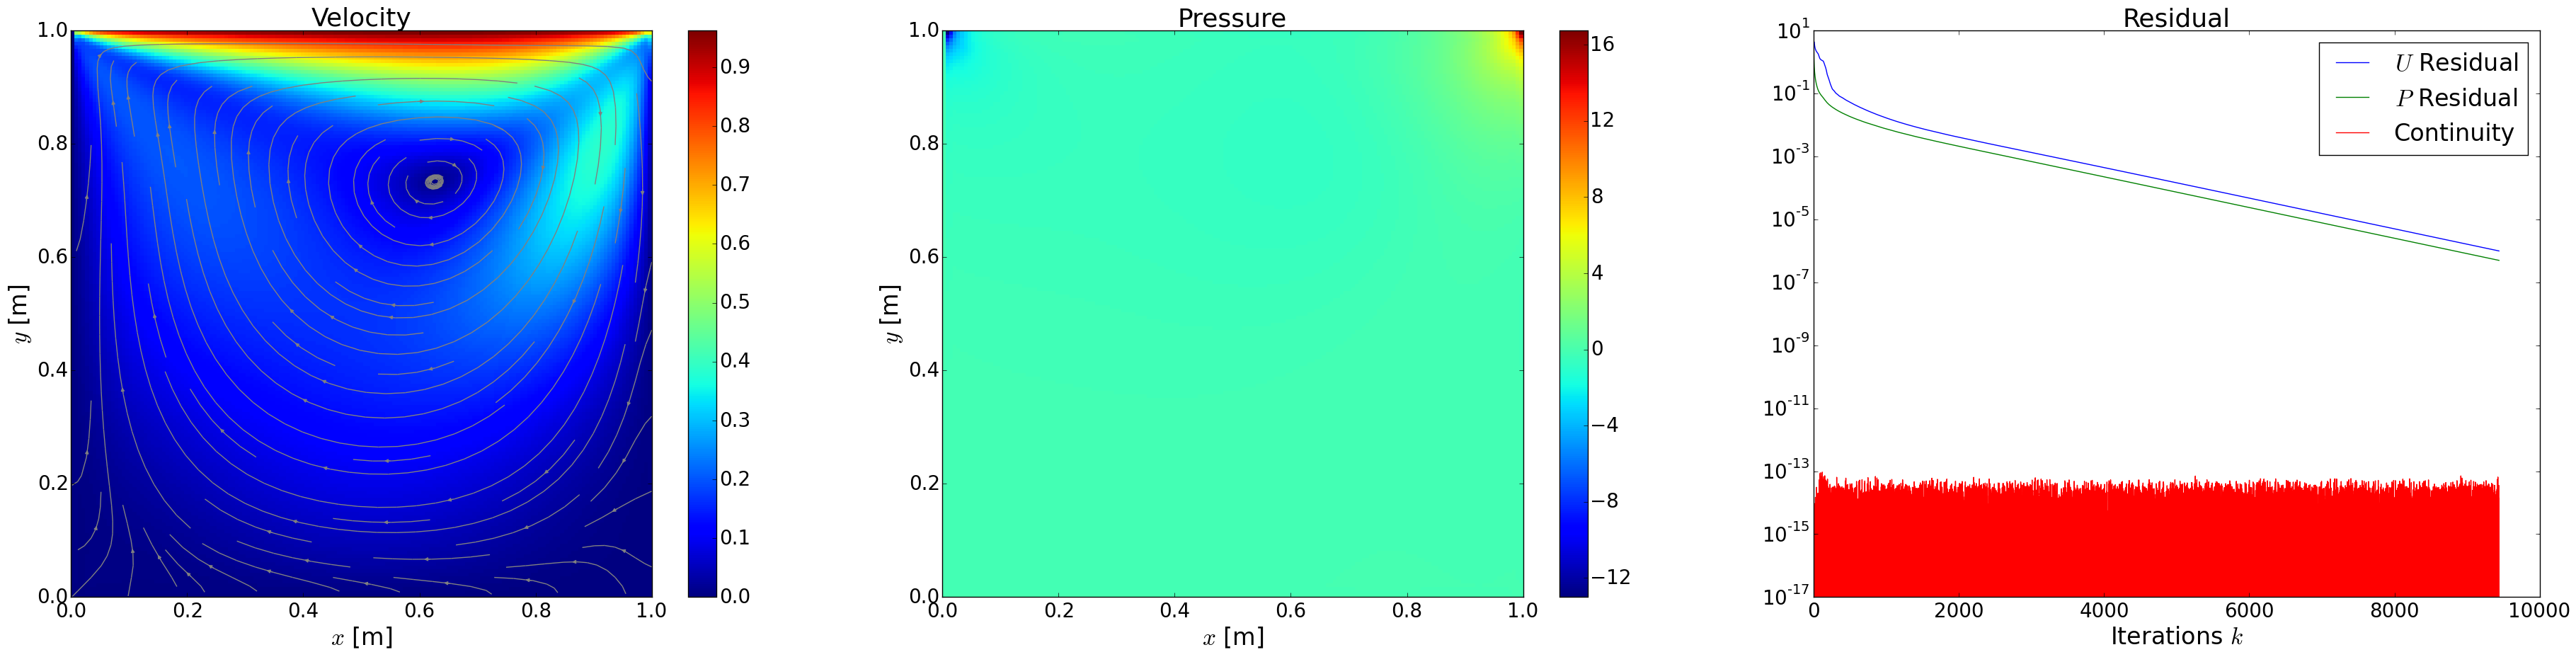
\includegraphics[width=\textwidth]{plot/solution10.png}
\footnotesize{\caption{Solution $Re$=10}\label{fig:solution10}}
\end{figure*}
\subsection*{Correction}

A correction is made such that a momentum conserving solution also conserves mass.
The velocity and pressure corrections are defined by equations \eqref{eq:pcorr} and \eqref{eq:ucorr}.
\begin{equation}\label{eq:pcorr}P = P\st + P'\end{equation}
\begin{equation}\label{eq:ucorr}u = u\st + u'\end{equation}

\subsubsection*{Velocity Correction}
From equations \eqref{eq:diffconvcoeff} and \eqref{eq:ucorr} the velocity correction is obtained.
\begin{equation}\label{eq:velcorr}a_P^uu_P' = -V\frac{P_e'-P_w'}{\delta x} + \sum\limits_n a_n^uu_n'\end{equation}
SIMPLE makes the simplification of dropping the term $\sum\limits_n a_n^u u_n'$ which leaves equation \eqref{eq:velcorrsimple} after cell face interpolations.
\[d = \frac{-V}{a_P^u}\]
\begin{equation}\label{eq:velcorrsimple}u_P' = d\frac{P_E'-P_W'}{\delta x};\hspace{1ex}v_P' = d\frac{P_N'-P_S'}{\delta y}\end{equation}

\subsubsection*{Pressure Correction}
The pressure correction is developed from the finite volume discretization of the mass conservation law \eqref{eq:massconservation}.
\begin{equation}(u_e-u_w)\delta y+(v_n-v_s)\delta x = 0\end{equation}
The velocity correction is applied giving equation \eqref{eq:massconservcorr}.
\begin{equation}\label{eq:massconservcorr}[(u_e+u_e')-(u_w+u_w')]\delta y+\end{equation}
\[[(v_n+v_n')-(v_s+v_s')]\delta x = 0\]
Substituting the corrected pressure for the corrected velocity equation \eqref{eq:velcorrsimple} gives the pressure correction coefficients detailed below.
%TODO: List pressure correction equation (?)
\[a_E^p = d_e \frac{\delta y}{\delta x};\hspace{1ex}a_W^p = d_w \frac{\delta y}{\delta x}\]
\[a_N^p = d_n\frac{\delta x}{\delta y};\hspace{1ex}a_S^p = d_s \frac{\delta x}{\delta y}\]
\[a_P^p = \sum_n a_n^P\]
\[b = \rho^{-1} [\delta y(u_e-u_w)+ \delta x (u_n-u_s)]\]
It can be observed that the coefficients are for that of a diffusion problem with nonuniform diffusion coefficient, leading to its stability.
However, diffusion problems require at least one Dirichlet boundary condition.
Since the driven cavity forgoes this requirement, there are infinitely many solutions to the pressure correction equation.
This can be avoided by placing a Dirichlet boundary condition on a single node as a reference point.
This would constrain the solution, keeping the pressure from straying from the reference pressure.

\begin{figure*}
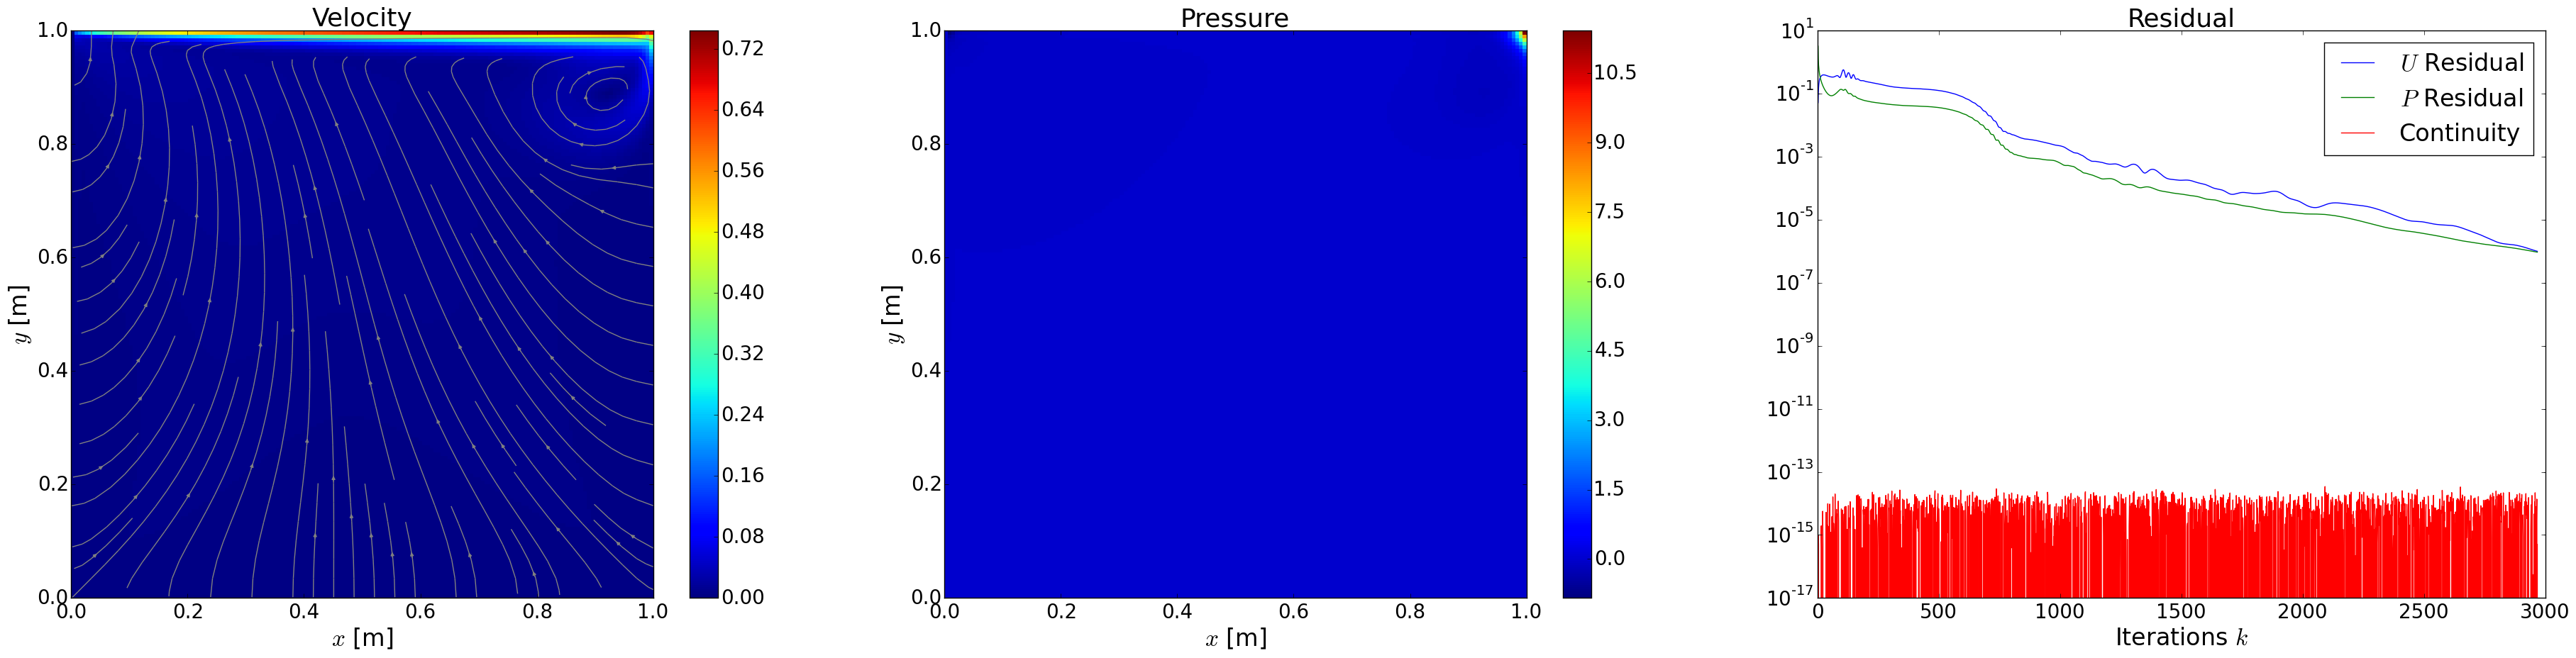
\includegraphics[width=\textwidth]{plot/solution100.png}
\footnotesize{\caption{Solution $Re$=100}\label{fig:solution100}}
\end{figure*}
\begin{figure*}
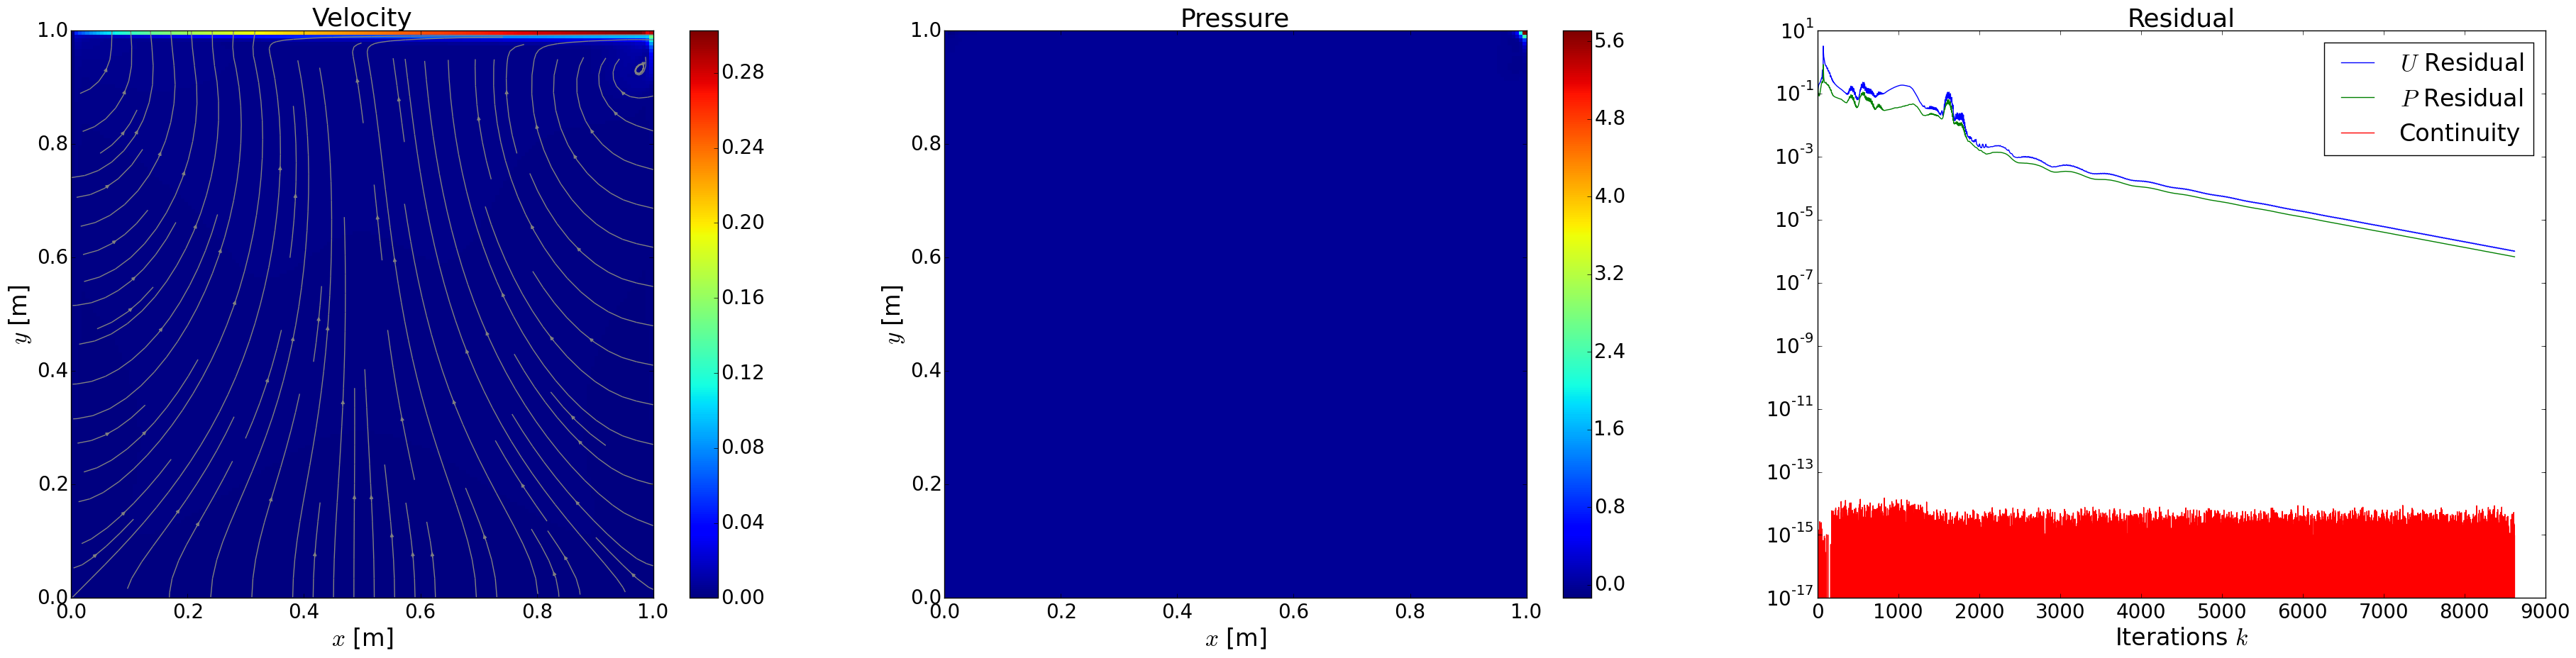
\includegraphics[width=\textwidth]{plot/solution400.png}
\footnotesize{\caption{Solution $Re$=400}\label{fig:solution400}}
\end{figure*}

\subsubsection*{Rhie-Chow Modification}
A limitation of the pressure gradient approximation is that oscillations in the pressure solution are not rejected.
A modification to the velocity correction in the pressure correction equation made by Rhie and Chow \eqref{eq:pcorrectionRC} introduces a term that prevents oscillations in the pressure field. 
\begin{equation}\label{eq:pcorrectionRC}u' =d(\nabla P' - {\overline\nabla P'})\end{equation}
\[\overline\nabla P_e = \frac{1}{2}\left(\nabla P_E + \nabla P_P\right)\]
While the term introduces error into the solution, it is $O(h^3)$ and will decrease much quicker than the error from other sources

\section*{Results}
A useful quantity known as the Reynolds number can be defined as the ratio \eqref{eq:reynolds} of intertial to viscous forces.
\begin{equation}\label{eq:reynolds}Re = \frac{\rho u}{\mu L^{-1}}\end{equation}
A problem where inertial effects are dominating such as fig. \ref{fig:solution400} has a high Reynolds number with very little diffusion of the velocity field, whereas fig. \ref{fig:solution10} has a low Reynolds number with a highly diffusive solution and a large resulting vortex.

\section*{Conclusion}
The flow field varied widely as the Reynolds number was increased.
The major results of reducing viscosity were the reduction in both the size and strength of the vortex as well as the migration of the vortex downstream.
This is consistent with the vortex being the result of shearing resulting from the North boundary.

The SIMPLE algorithm allowed easy computation of flow fields.
However, the algorithm was not robust, requiring tweaking to solver parameters to obtain convergence.
Since SIMPLE is a variant of Picard iteration, its convergence behavior is quite poor.
That said, SIMPLE does do a fairly good job at obtaining a solution without complicating the solver.
It is likely that SIMPLE would be outperformed by a solver based on Newton's method at the cost of code size.

\end{document}

